\documentclass[journal,15pt,twocolumn]{IEEEtran}
\usepackage[justification=centering,font={rm,md,scriptsize}]{caption}
\usepackage{graphicx}
\usepackage[margin=0.5in]{geometry}
\usepackage[cmex10]{amsmath}
\usepackage{amssymb}
\usepackage{array}
\usepackage{enumitem}
\usepackage{listings}
\usepackage{mathtools}
\usepackage{fancyvrb}
\usepackage{xcolor}
\usepackage{comment}
\usepackage{booktabs}
\usepackage{mathtools}
\usepackage{dirtree}
\usepackage{xcolor}
\usepackage{float}
%\usepackage{hyperref}
\newcounter{Chapcounter}
\newcommand\showmycounter{\addtocounter{Chapcounter}{1}\themycounter}
\newcommand{\chapter}[1] 
{ {\centering          
  \addtocounter{Chapcounter}{1} \large \textbf{Chapter \theChapcounter ~#1}}  
  \addcontentsline{toc}{section}{Chapter ~\theChapcounter~~ #1}    
  \setcounter{section}{0}
}
%%%%
\counterwithin{enumi}{section}
\counterwithin{equation}{enumi}
\counterwithin{figure}{enumi}
\renewcommand\thesection{\theChapcounter.\arabic{section}}
\renewcommand\thesectiondis{\theChapcounter.\arabic{section}}
\newcommand\figref{Fig.~\ref}
\setenumerate{label=\thesection.\arabic*}
\lstset{
  basicstyle=\ttfamily,
  columns=fullflexible,
  frame=single,
  breaklines=true,
  postbreak=\mbox{\textcolor{red}{$\hookrightarrow$}\space},
}
\providecommand{\mbf}{\mathbf}
\providecommand{\pr}[1]{\ensuremath{\Pr\left(#1\right)}}
\providecommand{\qfunc}[1]{\ensuremath{Q\left(#1\right)}}
\providecommand{\sbrak}[1]{\ensuremath{{}\left[#1\right]}}
\providecommand{\lsbrak}[1]{\ensuremath{{}\left[#1\right.}}
\providecommand{\rsbrak}[1]{\ensuremath{{}\left.#1\right]}}
\providecommand{\brak}[1]{\ensuremath{\left(#1\right)}}
\providecommand{\lbrak}[1]{\ensuremath{\left(#1\right.}}
\providecommand{\rbrak}[1]{\ensuremath{\left.#1\right)}}
\providecommand{\cbrak}[1]{\ensuremath{\left\{#1\right\}}}
\providecommand{\lcbrak}[1]{\ensuremath{\left\{#1\right.}}
\providecommand{\rcbrak}[1]{\ensuremath{\left.#1\right\}}}
\newcommand{\sgn}{\mathop{\mathrm{sgn}}}
\providecommand{\abs}[1]{\left\vert#1\right\vert}
\providecommand{\res}[1]{\Res\displaylimits_{#1}} 
\providecommand{\norm}[1]{\left\lVert#1\right\rVert}
\providecommand{\mtx}[1]{\mathbf{#1}}
\providecommand{\mean}[1]{E\left[ #1 \right]}
\providecommand{\fourier}{\overset{\mathcal{F}}{ \rightleftharpoons}}
\providecommand{\ztrans}{\overset{\mathcal{Z}}{ \rightleftharpoons}}
\providecommand{\system}{\overset{\mathcal{H}}{ \longleftrightarrow}}
\newcommand{\solution}{\noindent \textbf{Solution: }}
\newcommand{\cosec}{\,\text{cosec}\,}
\providecommand{\dec}[2]{\ensuremath{\overset{#1}{\underset{#2}{\gtrless}}}}
\newcommand{\myvec}[1]{\ensuremath{\begin{pmatrix}#1\end{pmatrix}}}
\newcommand{\mydet}[1]{\ensuremath{\begin{vmatrix}#1\end{vmatrix}}}
\providecommand{\gauss}[2]{\mathcal{N}\ensuremath{\left(#1,#2\right)}}
\newcommand*{\permcomb}[4][0mu]{{{}^{#3}\mkern#1#2_{#4}}}
\newcommand*{\perm}[1][-3mu]{\permcomb[#1]{P}}
\newcommand*{\comb}[1][-1mu]{\permcomb[#1]{C}}

\makeatletter
\newcommand*{\rom}[1]{\expandafter\@slowromancap\romannumeral #1@}
\makeatother

\let\vec\mathbf

\def\putbox#1#2#3{\makebox[0in][l]{\makebox[#1][l]{}\raisebox{\baselineskip}[0in][0in]{\raisebox{#2}[0in][0in]{#3}}}}
     \def\rightbox#1{\makebox[0in][r]{#1}}
     \def\centbox#1{\makebox[0in]{#1}}
     \def\topbox#1{\raisebox{-\baselineskip}[0in][0in]{#1}}
     \def\midbox#1{\raisebox{-0.5\baselineskip}[0in][0in]{#1}}

\begin{document}
%page heading start
\title{Digital Communication Through Simulation}
\author{Chirag Shah}
\maketitle
{\tableofcontents}
\bigskip
\textbf{Syntax for executing C program in Linux terminal} 
\begin{lstlisting}
gcc -o file_name file_name.c -I../include -lm
\end{lstlisting}
\textbf{Note}\\
include file has coeffs.f file which has to included with the execution command for C \vspace{2mm}
\textbf{Syntax for executing python program in Linux terminal }
\begin{lstlisting}
python3 file_name.py
\end{lstlisting}\vspace{2mm}
\chapter{Basics of Probability} 
\section {\textbf{Important Properties of the Probability Measure}}
\begin{align}
P(E^c)=1-P(E)
\end{align} 
where $E^c$ denotes the complement of $E$ This property implies that ,
\begin{align}
P(E^c)+P(E)=1
\end{align} 
\begin{align}
    P(\varnothing)=0
\end{align}
\begin{align}
    P(E_1 \cup E_2)=P(E_1)+P(E_2)-P(E_1 \cap E_2)
\end{align}
If two events $E_1$ and $E_2$ are mutually exclusive then ,
\begin{align}
         P(E_1 \cup E_2)=P(E_1)+P(E_2)
\end{align}
If 
\begin{align}
E_1	\subseteq E_2  
\end{align}
Then,
\begin{align}
P(E_1)\leq P(E_2)
\end{align}
This says that if event $E_1$ is contained in $E_2$ then occurrence of $E_1$ means $E_2$ has occurred but the converse is not true.
\section {\textbf{Conditional Probability}}
\textbf{Conditional probability} is known as the possibility of an event or outcome happening, based on the existence of a previous event or outcome.
It is calculated by multiplying the probability of the preceding event by the renewed probability of the succeeding, or conditional, event.\\
Let event $E_1$ has occurred but are actually interested in event $E_2$.\\
Knowing that of $E_1$ has occurred changes the probability of $E_2$ occurring.\\
The probability of $E_2$ occurring given that event $E_1$ has occurred.
\begin{align}
P(E_2 / E_1) &= 
\begin{cases}
\frac{P(E_2\bigcup E_1}{P(E_1)} & if P(E_1) \neq 0\\
0 & otherwise
\end{cases}
\end{align}
\section {\textbf{Uniform and Non-Uniform distribution}}
\textbf{The probability density function (PDF)} of the uniform distribution is given by, 
\begin{align}
    P(x) = \frac{1}{b-a}
\end{align}
For all the values
\begin{align}
	f(x) &=
	\begin{cases}
		\frac{1}{b-a} & a\le x \le b\\
		0 & x \le a / x \ge b
	\end{cases}
\end{align}
\textbf{The Cumulative distribution function (CDF)} of the uniform distribution is given by, 
\begin{align}
    F(x) = \frac{x-a}{b-a}
\end{align}
For all the values
\begin{align}
	F(x) &=
	\begin{cases}
            0 & x < a\\
		\frac{x-a}{b-a} & a \le x \le b\\
		1 & x > b 
	\end{cases}
\end{align}
\textbf{The Gaussian distribution function} of the Non uniform distribution is given by,
\begin{align}
    f(x,\mu,\sigma) = \frac{1}{\sigma\sqrt{2\pi}} \exp \left( \frac{-(x-\mu)^2}{2\sigma^2} \right)
\end{align}
\chapter{Two Dice}
\section {\textbf{Sum of Independant Random Variables}}
\textbf{Introduction} \\ \vspace{2mm}
Let  $X$ and $Y$ be random variables.\\The distribution of their sum is given by,
\begin{align}
    T=X+Y
\end{align} 
To determine the distribution of $T$ we need to calculate 
\begin{align}
    f_T(t)=P(t=t)=P(X+Y=t) 
\end{align}
Which we can do by summing the joint p.m.f. over the appropriate values:
\begin{align}
\sum_{(x,y):x+y=t}^{}f(x,y)
\end{align}
\textbf{Example:}\\ \vspace{2mm}
To calculate the total number of bets that Xavier and Yolanda win,\\
By calculating $P(X+Y=T)$ for $t$=0,1,2,3,....,8.\\
The probabilities that we would need to sum for $t$=4 are highlighted in the joint p.m.f. table below
\begin{figure}[H]
\centering
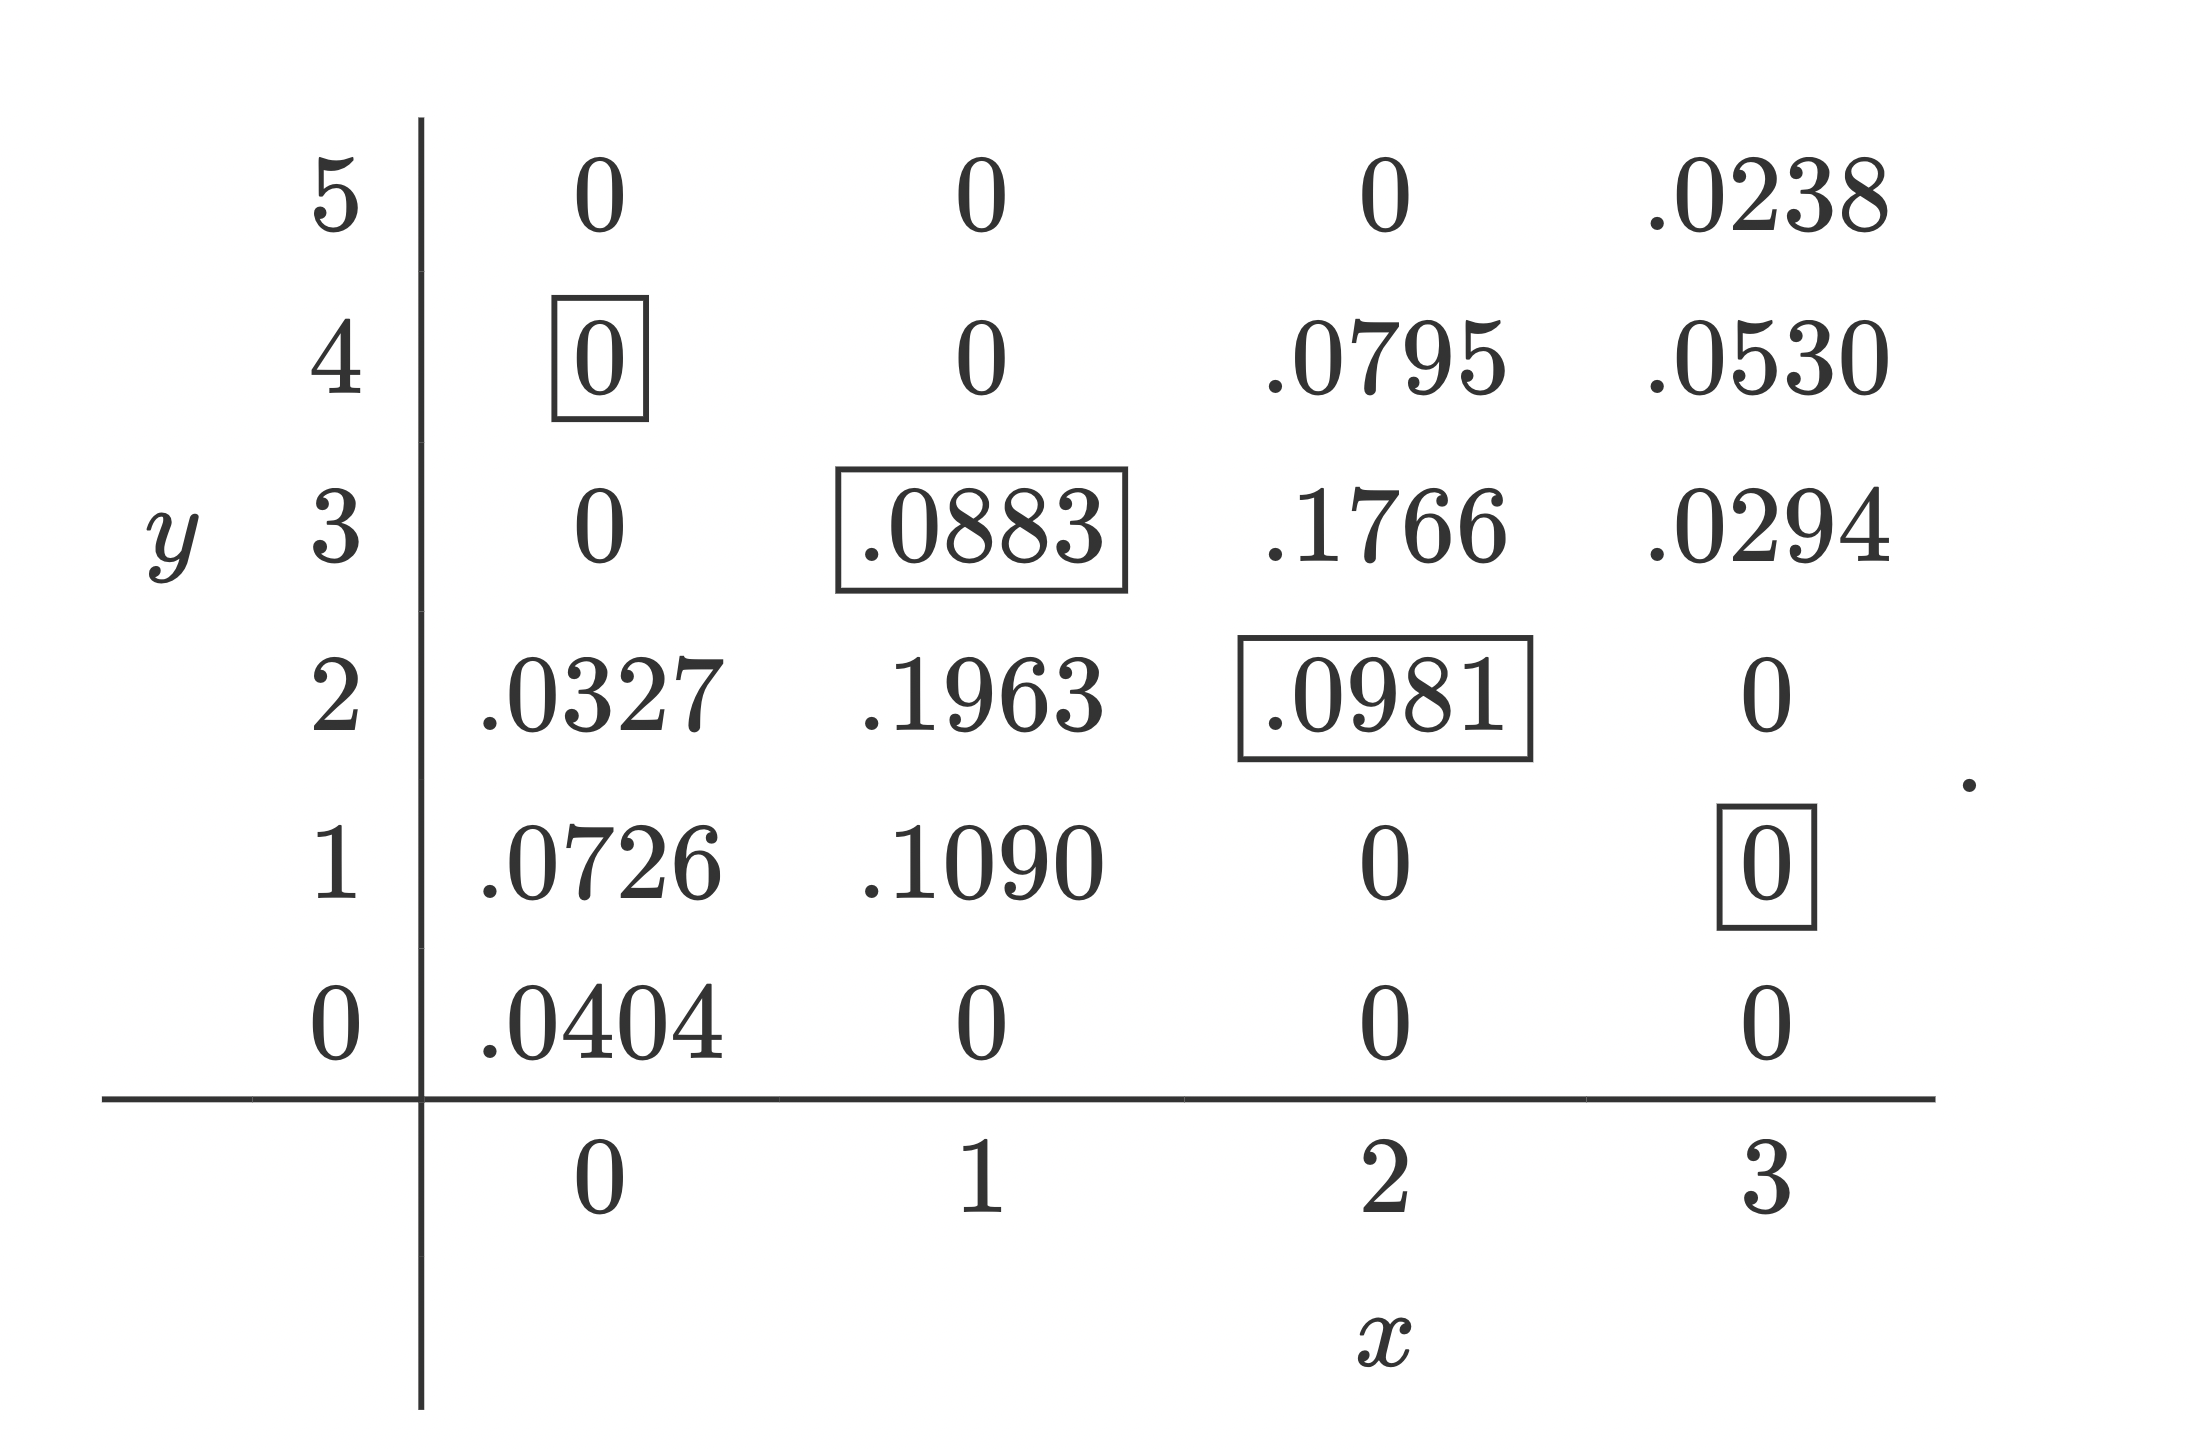
\includegraphics[width=\columnwidth]{./figs/chapter2/win_table.png}
\caption{Joint p.m.f fot $t$=4}
\label{joint_pmf}
\end{figure}
For a fixed value of $t$, $x$ determines the value of $y$ and and vice versa,\\
In General,
\begin{align}
    y=t-x\\
\end{align}
Using the above equation 
\begin{align}
f_T(t)= \sum_{x}^{}f(x,t-x)
\end{align}
This is the general equation for the p.m.f. of the sum $T$. \\ \vspace{2mm}
\textbf{For Independent random variables}\\
Let $X$ and $Y$ be independent random variables.\\
Then, the p.m.f. of $T$ 
\begin{align}
    T=X+Y
\end{align}
 Its convolution of the p.m.f.s of $X$ AND $Y$ is
\begin{align}
 f_T=f_X*f_Y
\end{align}
The convolution operator (*) is defined as
\begin{align}
    f_T(t)= \sum_{x}^{}f(x) \mathord{\cdot} f_Y(t-x)
\end{align}
 The joint distribution is the product of the marginal distributions \\
 We have,
 \begin{align}
    f_T(t)= f_X(x)\mathord{\cdot} f_Y(t-x)
\end{align}
Two dice, one blue and one grey, are thrown at the same time.   The event defined by the sum of the two numbers appearing on the top of the dice can have 11 possible outcomes 2, 3, 4, 5, 6, 6, 8, 9, 10, 11 and 12.  A student argues that each of these outcomes has a probability $\frac{1}{11}$.  Do you agree with this argument?  Justify your answer.
%
\begin{enumerate}
\item  {\em The Uniform Distribution: }Let $X_i \in \cbrak{1,2,3,4,5,6}, i = 1,2,$ be the random variables representing the outcome for each die.  Assuming the dice to be fair, the probability mass function (pmf) is expressed as 
\begin{align}
\label{eq:pmf}
p_{X_i}(n) = \pr{X_i = n} = 
\begin{cases}
\frac{1}{6} & 1 \le n \le 6
\\
0 & otherwise
\end{cases}
\end{align}
The desired outcome is
\begin{align}
\label{eq:out_dice}
X &= X_1 + X_2,
\\
\implies X &\in \cbrak{1,2,\dots,12}
\end{align}
%
The objective is to show that
\begin{align}
p_X(n) \ne \frac{1}{11}
\label{eq:dice_null}
\end{align}
\item {\em Convolution: }\\
From \eqref{eq:out_dice},
\begin{align}
p_X(n) &= \pr{X_1 + X_2 = n} = \pr{X_1  = n -X_2}
\\
&= \sum_{k}^{}\pr{X_1  = n -k | X_2 = k}p_{X_2}(k)
\label{eq:sum_x}
\end{align}%
after unconditioning.  $\because X_1$ and $X_2$ are independent,
\begin{multline}
\pr{X_1  = n -k | X_2 = k} 
\\
= \pr{X_1  = n -k} = p_{X_1}(n-k)
\label{eq:indp_x}
\end{multline}
From \eqref{eq:sum_x} and \eqref{eq:indp_x},
\begin{align}
p_X(n) = \sum_{k}^{}p_{X_1}(n-k)p_{X_2}(k) = p_{X_1}(n)*p_{X_2}(n)
\label{eq:convolution_x}
\end{align}
where $*$ denotes the convolution operation. 
%\cite{proakis_dsp}.  
Substituting from \eqref{eq:pmf}
in \eqref{eq:convolution_x},
\begin{align}
p_X(n) = \frac{1}{6}\sum_{k=1}^{6}p_{X_1}(n-k)= \frac{1}{6}\sum_{k=n-6}^{n-1}p_{X_1}(k)
\label{eq:convolution_x_x1}
\end{align}
\begin{align}
\because p_{X_1}(k) &= 0, \quad k \le 1, k \ge 6.
\end{align}
From \eqref{eq:convolution_x_x1},
%
\begin{align}
p_X(n) &= 
\begin{cases}
0 & n < 1
\\
\frac{1}{6}\sum_{k=1}^{n-1}p_{X_1}(k) &  1 \le n-1 \le  6
\\
\frac{1}{6}\sum_{k=n-6}^{6}p_{X_1}(k) & 1 < n-6 \le 6
\\
0 & n > 12
\end{cases}
\label{eq:convolution_x_exp}
\end{align}
Substituting from \eqref{eq:pmf} in \eqref{eq:convolution_x_exp},
\begin{align}
p_X(n) &= 
\begin{cases}
0 & n < 1
\\
\frac{n-1}{36} &  2 \le n \le  7
\\
\frac{13-n}{36} & 7 < n \le 12
\\
0 & n > 12
\end{cases}
\label{eq:convolution_x_final}
\end{align}
satisfying \eqref{eq:dice_null}.
\item {\em The $Z$-transform: }
The $Z$-transform of $p_X(n)$ is defined as 
%\cite{proakis_dsp}
\begin{align}
P_X(z) = \sum_{n = -\infty}^{\infty}p_X(n)z^{-n}, \quad z \in \mathbb{C}
\label{eq:z_trans}
\end{align}
%
From \eqref{eq:pmf} and \eqref{eq:z_trans}, 
\begin{align}
P_{X_1}(z) =P_{X_2}(z) &= \frac{1}{6}\sum_{n = 1}^{6}z^{-n}
\\
&=\frac{z^{-1}\brak{1-z^{-6}}}{6\brak{1-z^{-1}}}, \quad \abs{z} > 1
\label{eq:z_trans_x}
\end{align}
upon summing up the geometric progression.  
\begin{align}
\because p_X(n) &= p_{X_1}(n)*p_{X_2}(n),
\\
P_X(z) &= P_{X_1}(z)P_{X_2}(z)
\label{eq:z_fact_pod}
\end{align}
The above property follows from Fourier analysis and is fundamental to signal processing. 
%\cite{proakis_dsp}. 
From \eqref{eq:z_trans_x} and \eqref{eq:z_fact_pod},
\begin{align}
P_X(z) &= \cbrak{\frac{z^{-1}\brak{1-z^{-6}}}{6\brak{1-z^{-1}}}}^2
\\
&= \frac{1}{36}\frac{z^{-2}\brak{1-2z^{-6}+z^{-12}}}{\brak{1-z^{-1}}^2}
\label{eq:z_fact}
\end{align}
Using the fact that 
%\cite{proakis_dsp}
\begin{align}
p_X(n-k) &\system{Z}P_X(z)z^{-k},
\\
nu(n)&\system{Z} \frac{z^{-1}}{\brak{1-z^{-1}}^2}
\end{align}
after some algebra, it can be shown that
%{\tiny
\begin{multline}
\frac{1}{36}\lsbrak{\brak{n-1}u(n-1) - 2 \brak{n-7}u(n-7)}
\\
\rsbrak{ +\brak{n-13}u(n-13)}
\\
\system{Z}
\frac{1}{36}\frac{z^{-2}\brak{1-2z^{-6}+z^{-12}}}{\brak{1-z^{-1}}^2}
\label{eq:z_fact_fun}
\end{multline}
%}
where 
\begin{align}
u(n) =
\begin{cases}
1 & n \ge 0
\\
0 & n < 0
\end{cases}
\end{align}
From \eqref{eq:z_trans}, \eqref{eq:z_fact} and \eqref{eq:z_fact_fun}
\begin{multline}
p_{X}(n) = \frac{1}{36}\lsbrak{\brak{n-1}u(n-1) 
}
\\
\rsbrak{- 2 \brak{n-7}u(n-7)+\brak{n-13}u(n-13)}
\end{multline}
which is the same as \eqref{eq:convolution_x_final}.  Note that  \eqref{eq:convolution_x_final} can be obtained from \eqref{eq:z_fact_fun} using contour integration as well.
% \cite{proakis_dsp}.  
\item 
The experiment of rolling the dice was simulated using Python for 10000 samples.  These were generated using Python libraries for uniform distribution. The frequencies for each outcome were then used to compute the resulting pmf, which  is plotted in Figure \ref{fig:dice}.  The theoretical pmf obtained in \eqref{eq:convolution_x_final} is plotted for comparison.  
%
\begin{figure}[H]
\centering
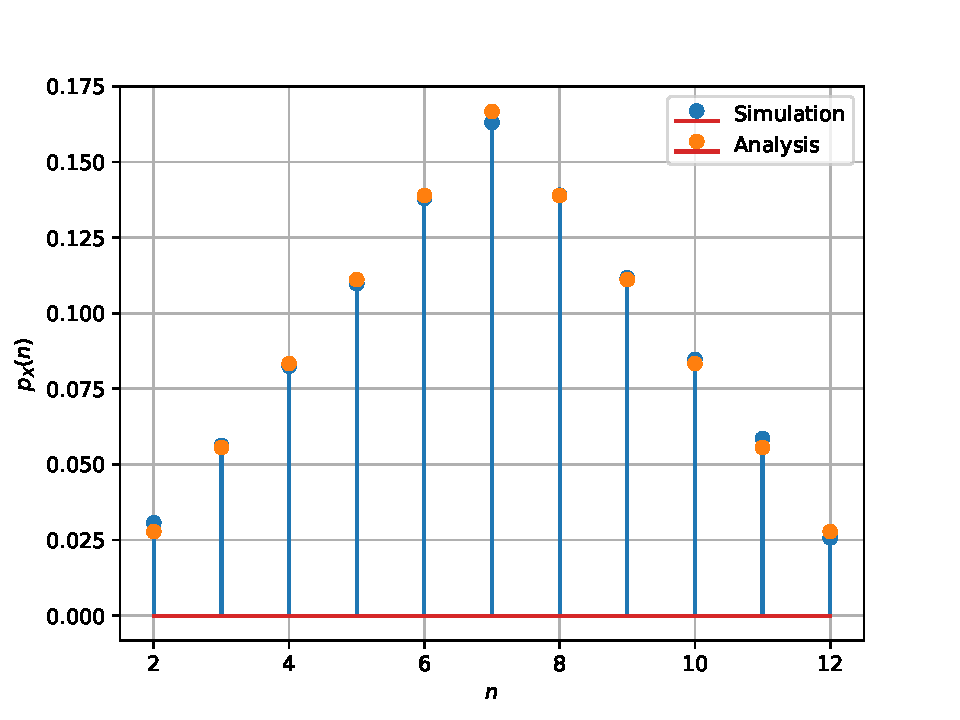
\includegraphics[width=\columnwidth]{./figs/chapter2/two_dices.pdf}
\caption{Plot of $p_X(n)$.  Simulations are close to the analysis. }
\label{fig:dice}
\end{figure}
\item Code of above solution 
\begin{lstlisting}
/codes/chapter2/two_dice.py
\end{lstlisting}
\item For executing python program in linux terminal
\begin{lstlisting}
python3 two_dice.py
\end{lstlisting}
\end{enumerate}

\chapter{Random Numbers}
\section{\textbf{Uniform Random Numbers}}
It's just a random number where each possible number is just as likely as any other possible number.\\ 
Example :  A fair die is a uniform random number generator for numbers between 1 and 6 inclusive.\\
\textbf{The probability density function }of the uniform distribution is given by,
\begin{align}
    P(x) = \frac{1}{b-a}
\end{align}
\begin{align}
	f(x) &=
	\begin{cases}
		\frac{1}{b-a} & a\le x \le b\\
		0 & x \le a / x \ge b
	\end{cases}
\end{align}
\textbf{The Cumulative distribution function} of the uniform distribution is given by,
\begin{align}
    F(x) = \frac{x-a}{b-a}
\end{align}
\begin{align}
	F(x) &=
	\begin{cases}
            0 & x < a\\
		\frac{x-a}{b-a} & a \le x \le b\\
		1 & x > b 
	\end{cases}
\end{align}
Let $U$ be a uniform random variable between 0 and 1.
\begin{enumerate}
\item Generate $10^6$ samples of $U$ using a C program and save into a file called uni.dat .
\label{prob:uni_gen}
\\
\solution Download the following files and execute the  C program.
\begin{lstlisting}
codes/chapter3/gen_samp.c
\end{lstlisting} 
\item For executing C program in linux terminal 
\begin{lstlisting}
gcc -o gen_samp gen_sam.c -I../include -lm
\end{lstlisting}
%
\item
Load the uni.dat file into python and plot the empirical CDF of $U$ using the samples in uni.dat. The CDF is defined as
\begin{align}
F_{U}(x) = \pr{U \le x}
\end{align}
\\
\solution  The following code plots \figref{fig:uni_cdf}
\begin{lstlisting}
codes/chapter3/cdf_plot.py
\end{lstlisting}
\begin{figure}[H]
\centering
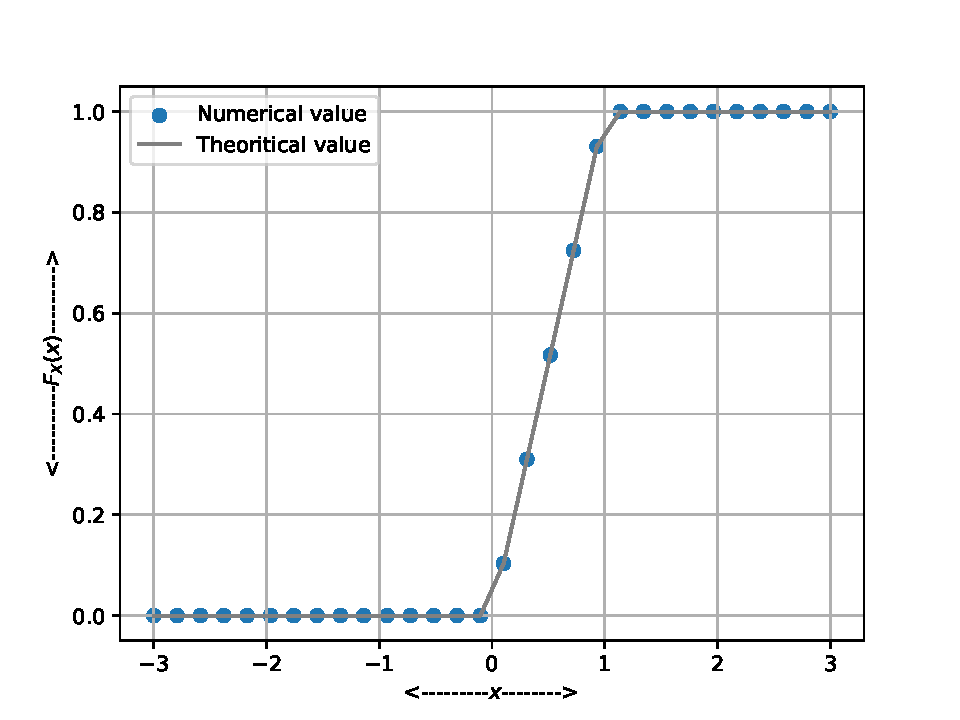
\includegraphics[width=\columnwidth]{./figs/chapter3/cdf_plot.pdf}
\caption{The CDF of $U$}
\label{fig:uni_cdf}
\end{figure}

%
\item
Find a  theoretical expression for $F_{U}(x)$.\\
\solution \\
$F_{U}(x)$ is defined as $\int_{-\infty}^{x} f_{U}(x)\,dx$
\begin{align} 
 F_{U}(x)= \int_{-\infty}^{x} f_{U}(x)\,dx
\end{align}
For the random variable which is uniform throughout $U$,\\ $f_{U}(x)$ is 
\begin{align}
	f_U(x) &= 
	\begin{cases}
	1 &  0 \le x \le  1
	\\
	0 & elsewhere
	\\
	\end{cases}
\end{align}
Substituting it, we get
\begin{align}
	F_U(x) &= 
	\begin{cases}
	0 & x < 0
	\\	
	x & 0 \le x \le  1
	\\
	1 & x > 0
	\\
	\end{cases}
	\label{eq:cdf_uniform}
\end{align}
\item To find Mean, \\ 
The mean of $U$ is given by,
%
\begin{equation}
E\sbrak{U} = \frac{1}{N}\sum_{i=1}^{N}U_i
\end{equation}
%
\item To find variance,\\
The variance of  $U$ is given by,
%
\begin{equation}
\text{var}\sbrak{U} = E\sbrak{U- E\sbrak{U}}^2 
\end{equation}

Write a C program to  find the mean and variance of $U$.\\ \vspace{2mm}
\solution Source code is given below
\begin{lstlisting}
codes/chapter3/gen_samp.c
\end{lstlisting}
\textbf {Output} \vspace{2mm}
\begin{lstlisting}
Mean is: 0.500031 
Variance is: 0.083247
\end{lstlisting}
\item Verify your result theoretically given that
%
\begin{equation}
E\sbrak{U^k} = \int_{-\infty}^{\infty}x^kdF_{U}(x)
\end{equation}\\
\solution For a random variable $X$, \\ Mean $\mu_X$ is given by,
\begin{align}
	\label{eq:mean_rand}
	\mu_X & = \int_{-\infty}^{\infty}xdF_{U}(x) = E\sbrak{X}
\end{align}  
Substituting from \eqref{eq:cdf_uniform} $F_U(x)$ in the above equations, we get
\begin{align} 
	 E\sbrak{X}=\mu_U &= \frac{1}{2} 
  \end{align}
\vspace{2mm}Variance $\sigma_X^2$ is given by,
\begin{align}
\label{eq:x_var}
	\sigma_X^2 &= \int_{-\infty}^{\infty}x^2dF_{U}(x) - \mu_X^2 = E\sbrak{X^2} - \mu_X^2 
 \end{align}
Substituting from \eqref{eq:cdf_uniform} $F_U(x)$ in the above equations, we get
\begin{align} 
	E\sbrak{X^2} - \mu_X^2 =\sigma_U^2 &= \frac{1}{12}
\end{align}  \vspace{2mm}

\end{enumerate}
\section{\textbf{Central Limit Theorem}}
The central limit theorem states that whenever a random sample of size n is taken from any distribution with mean and variance, then the sample mean will be approximately normally distributed with mean and variance. The larger the value of the sample size, the better the approximation to the normal.\\
\textbf{Formula}
\begin{align}
    Z = \frac{ \Bar{x} -\mu}{\frac{\sigma}{\sqrt{n}}} 
\end{align}
\begin{enumerate}
%
%
\item
Generate $10^6$ samples of the random variable
%
\begin{equation}
X = \sum_{i=1}^{12}U_i -6
\end{equation}
%
using a C program, where $U_i, i = 1,2,\dots, 12$ are  a set of independent uniform random variables between 0 and 1
and save in a file called gau.dat\\
\solution Source code
\begin{lstlisting}
codes/chapter3/gau_cdf_pdf.c
\end{lstlisting}
\textbf{Output}
\begin{lstlisting}
Mean is : 0.000630
Variance is : 1.000150
\end{lstlisting}
%
\item
Load gau.dat in python and plot the empirical CDF of $X$ using the samples in gau.dat. What properties does a CDF have?
\\
\solution 
The properties of a CDF are 
\begin{eqnarray}
       \frac{dF_X(x)}{dx} \ge 0 \\
        F_X(\infty) = 0\\
	F_X(-\infty) = 1
\end{eqnarray}
Below code for generating CDF of $X$
\begin{lstlisting}
codes/chapter3/gau_cdf.py
\end{lstlisting}
The CDF of $X$ is shown in fig below
\begin{figure}[H]
\centering
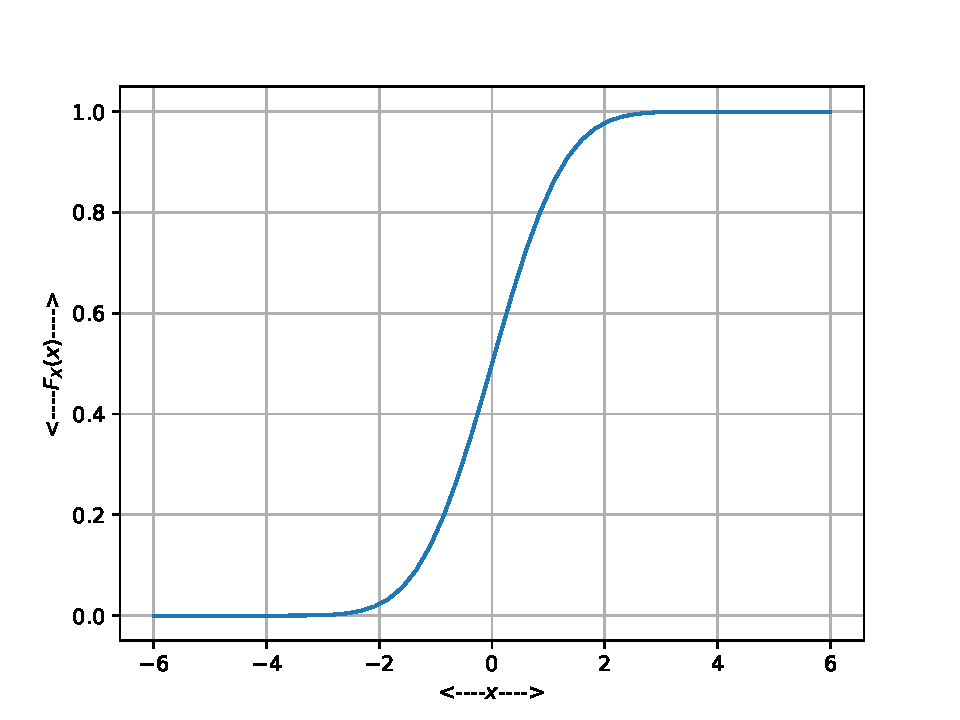
\includegraphics[width=\columnwidth]{./figs/chapter3/gau_cdf.pdf}
\caption{The CDF of $X$}
\label{fig:gauss_cdf}
\end{figure}

\item
Load gau.dat in python and plot the empirical PDF of $X$ using the samples in gau.dat. \\The PDF of $X$ is defined as,
\begin{align}
p_{X}(x) = \frac{d}{dx}F_{X}(x)
\label{eq:cdf_to_pdf}
\end{align}
What properties does the PDF have?
\\
\solution The properties of PDF are
\begin{eqnarray}
	f_X(x) \ge 0\\
	\int_{-\infty}^{\infty} f_X(x) \,dx = 1
\end{eqnarray}

Below code for generating PDF of $X$
\begin{lstlisting}
codes/chapter3/gau_pdf.py
\end{lstlisting}
The PDF of $X$ is shown in fig below
\begin{figure}[H]
\centering
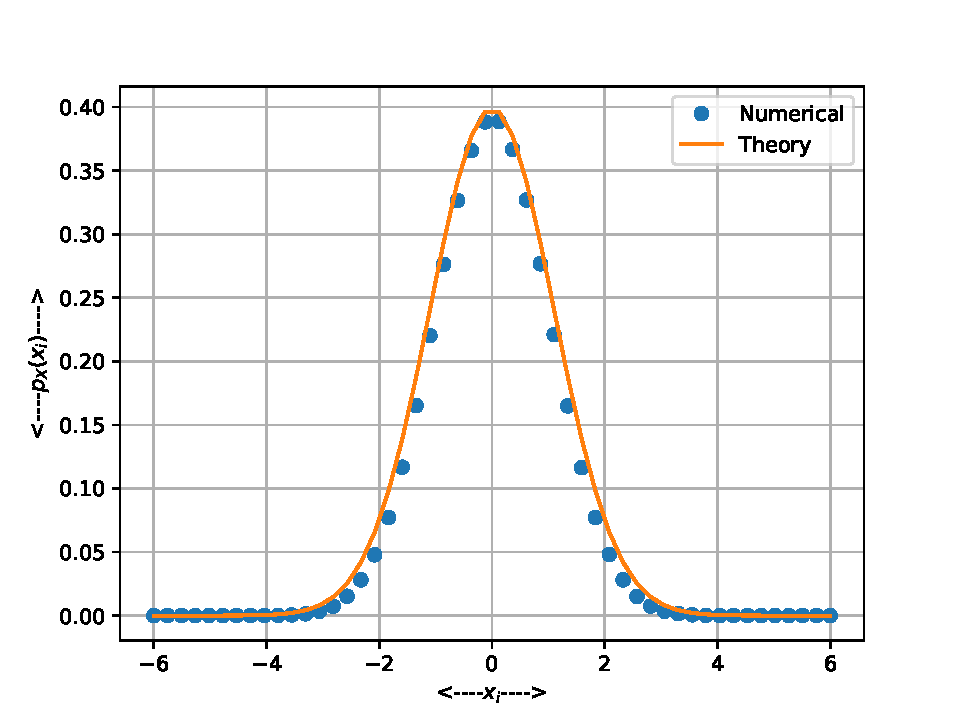
\includegraphics[width=\columnwidth]{./figs/chapter3/gau_pdf.pdf}
\caption{The PDF of $X$}
\label{fig:gauss_pdf}
\end{figure}

\item Find the mean and variance of $X$ by writing a C program.
\solution Below code gives you mean and variance of $X$
\begin{lstlisting}
codes/chapter3/gau_cdf_pdf.c
\end{lstlisting}
\textbf{Output} 
\begin{lstlisting}
Mean is : 0.000630
Variance is : 1.000150
\end{lstlisting}
\item Given that 
\begin{align}
p_{X}(x) = \frac{1}{\sqrt{2\pi}}\exp\brak{-\frac{x^2}{2}}, -\infty < x < \infty,
\end{align}
repeat the above exercise theoretically.\\
\solution Substituting the below equation in \eqref{eq:mean_rand},

\begin{align}
	\label{eq:mean_rand}
	 E\sbrak{X}=\mu_X & = \int_{-\infty}^{\infty}xdF_{U}(x)
\end{align}  
We get,
\begin{flalign}
	 E\sbrak{X}=\mu_X &= \int_{-\infty}^{\infty} \frac{x}{\sqrt{2\pi}}\exp\brak{-\frac{x^2}{2}} \,dx&\\
	\mu_X &= \frac{1}{\sqrt{2\pi}}\left[-\exp\brak{-\frac{x^2}{2}}\right]_{-\infty}^{\infty}&\\  
	 E\sbrak{X}=\mu_X &= 0
\end{flalign}
Substituting the below equation in \eqref{eq:mean_rand},
\begin{align}
\label{eq:x_var}
	\sigma_X^2 &= \int_{-\infty}^{\infty}x^2dF_{U}(x) - \mu_X^2 = - \mu_X^2 
 \end{align}
\begin{flalign}
	\sigma_X^2 &= \int_{-\infty}^{\infty} x^2\frac{1}{\sqrt{2\pi}}\exp\brak{-\frac{x^2}{2}} \,dx-0&\\ \nonumber
	 \sigma_X^2 &= \frac{2}{\sqrt{\pi}} \int_{0}^{\infty} x^2\frac{1}{\sqrt{2\pi}}\exp\brak{-\frac{x^2}{2}} \,dx&\\	\nonumber\\
 \intertext{Let a = $\frac{x^2}{2}$ and using gama function,} 
 \intertext{We have,}
	&\\	\nonumber
	\sigma_X^2 &= \frac{2}{\sqrt{\pi}} \int_{0}^{\infty} t^{\frac{3}{2}-1}\exp\brak{-t} \,dt&\\
	 \Gamma(x) &= \int_{0}^{\infty} e^{-z} z^{x-1}  \, \mathrm{d}x \,&\\
	\sigma_X^2 &= 2\frac{1}{\sqrt{\pi}}\frac{\sqrt{\pi}}{2}=1&\\	\nonumber
	& E\sbrak{X^2}=\sigma_X^2=1	
\end{flalign}
%
\end{enumerate}
\section{From Uniform to Other}
\begin{enumerate}
%
\item
Generate samples of 
%
\begin{equation}
V = -2\ln\brak{1-U}
\end{equation}
%
and plot its CDF. \\
\solution \\
Using uni.dat the CDF of $V$ is plotted in \figref{fig:log_uni_cdf} \\
\textbf{Code for loading and plotting graph from uni.dat }
\begin{lstlisting}
codes/chapter3/cdf_v.py
\end{lstlisting}
\begin{figure}[H]
\centering
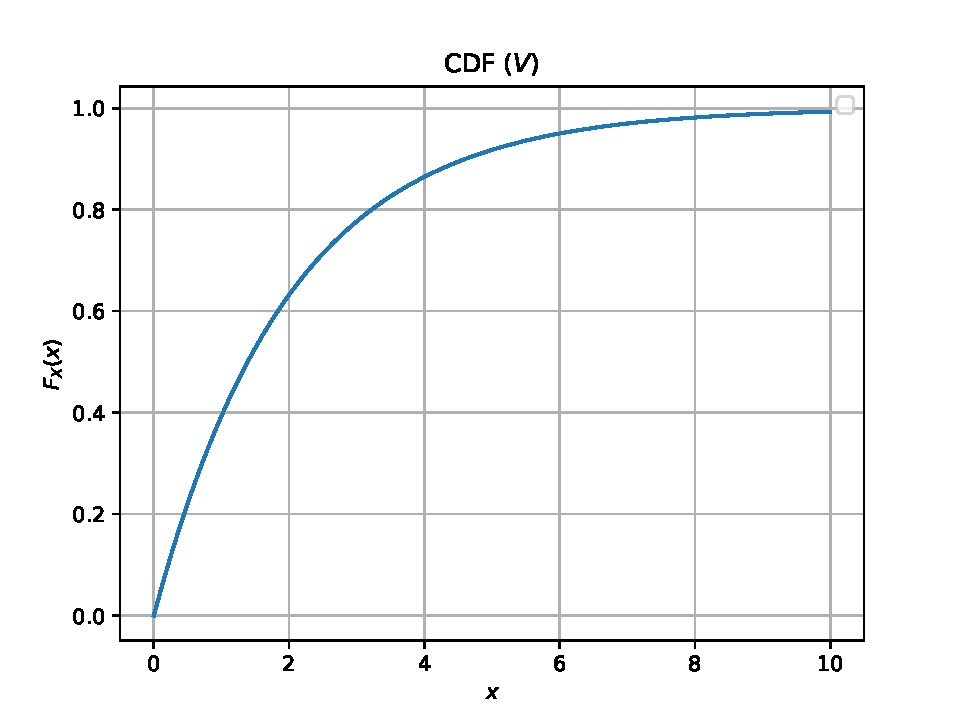
\includegraphics[width=\columnwidth]{./figs/chapter3/cdf_v.pdf}
\caption{The CDF of $V$}
\label{fig:log_uni_cdf}
\end{figure}
\item Find a theoretical expression for $F_V(x)$.
\begin{flalign}
	F_V(w) &= P(V < w)&\\
 \intertext{We know that ,}
        &V = -2\ln\brak{1-U}\\
        \intertext{Substituting the above eq in $F_V(w)$ }
        \intertext{We get,}
	&F_V(w)= P(-2\ln\brak{1-U}) < w)&\\
        &= P(\ln(1-U) \ge -\frac{w}{2})\\
        \intertext{Taking log to exp}
        &= P( 1-U \ge \exp\brak{-\frac{w}{2}})\\
	&= P(U < 1 - \exp\brak{\frac{-w}{2}})&\\
 \intertext{Now ,}
	&F_V(w)= F_U(1 - e^{\frac{-w}{2}})
\end{flalign}
$F_U(x)$ is dedined as,
\begin{align}
	F_U(x) &= 
	\begin{cases}
	   1 & x > 0
	\\	
	x & 0 \le x \le  1
	\\
	0 & x < 0
	\\
	\end{cases}
\end{align}
 Using the above equation in (2.3.2.7)\\
$F_V(w)$ is defined as 
\begin{align}
	F_V(w) &=
	\begin{cases}
		 1 - e^{\frac{-w}{2}} & w \ge 0\\
		0 & w < 0
	\end{cases}
\end{align} 
%
%\item
%Generate the Rayleigh distribution from Uniform. Verify your result through graphical plots.
\end{enumerate}

\section{Triangular Distribution}
%

\begin{enumerate}
\item Find the theoretical expressions for the PDF and CDF of $T$.\\
\solution The CDF and PDF of T is given by, \\
  For PDF \\
  Using ,
 \begin{align}
	f_U(x) &= 
	\begin{cases}
	1 &  0 \le x \le  1
	\\
	0 & elsewhere
	\\
	\end{cases}
 \end{align}
 We have,
\begin{align}
	f_T(x) &=
	\begin{cases}
		x & 0 \le x \le 1\\
		2-x & 1 \le x \le 2\\
		0 & \text{other wise}
	\end{cases}
\end{align}
For CDF of $T$ \\
Using,
\begin{align} 
 F_{U}(x)= \int_{-\infty}^{x} f_{U}(x)\,dx
\end{align}
We have,
\begin{align}
	F_T(x) &=
	\begin{cases} 
            1 & x > 2\\
            2x-\frac{x^2}{2}-1 & 1 \le x \le 2\\
            \frac{x^2}{2} & 0 \le x \le 1\\
		0 & \text{other wise}
	\end{cases}
\end{align}
\item Generate 
	\begin{align}
		T = U_1+U_2
	\end{align}\\
\solution C code is given below  
\begin{lstlisting}
codes/chapter3/two_uni.c
\end{lstlisting}
\item Find the CDF of $T$.\\
\solution After running above C code push the u1.dat and u2.dat in python code given below.
\begin{lstlisting}
codes/chapter3/two_uni_cdf.py
\end{lstlisting}
Below fig shows the CDF of T.
\begin{figure}[H]
\centering
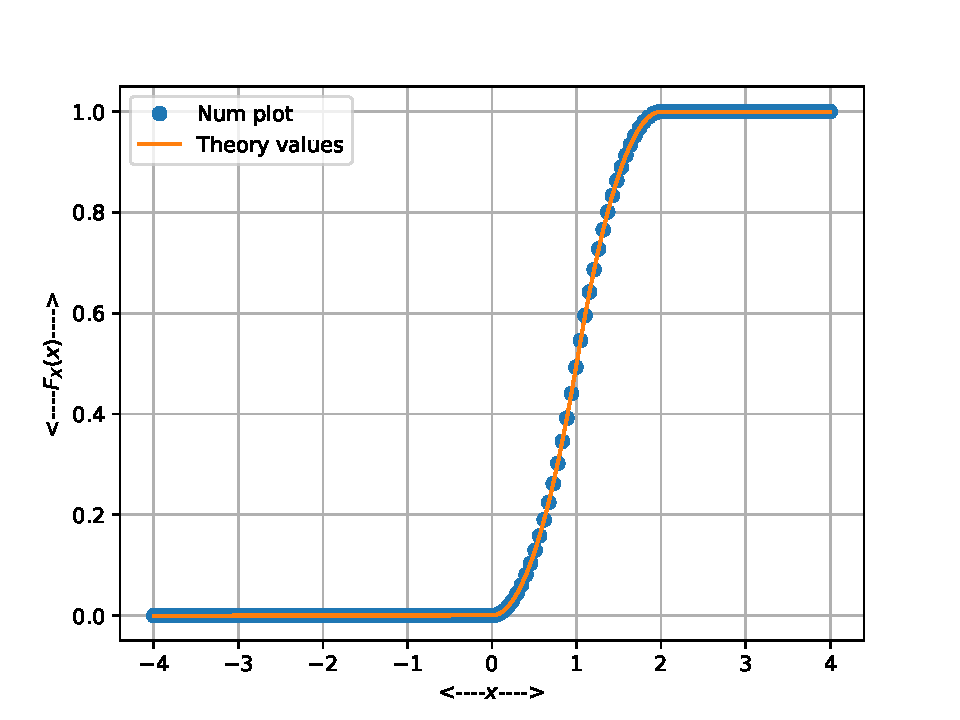
\includegraphics[width=\columnwidth]{./figs/chapter3/tri_dist_cdf.pdf}
\caption{The CDF of $T$}
\label{fig:tri_cdf}
\end{figure}
\item Find the PDF of $T$.\\
\solution The PDF of $T$ is plotted in \figref{fig:tri_pdf} using the code below
\begin{lstlisting}
codes/chapter3/two_uni_pdf.py
\end{lstlisting}
\begin{figure}[H]
\centering
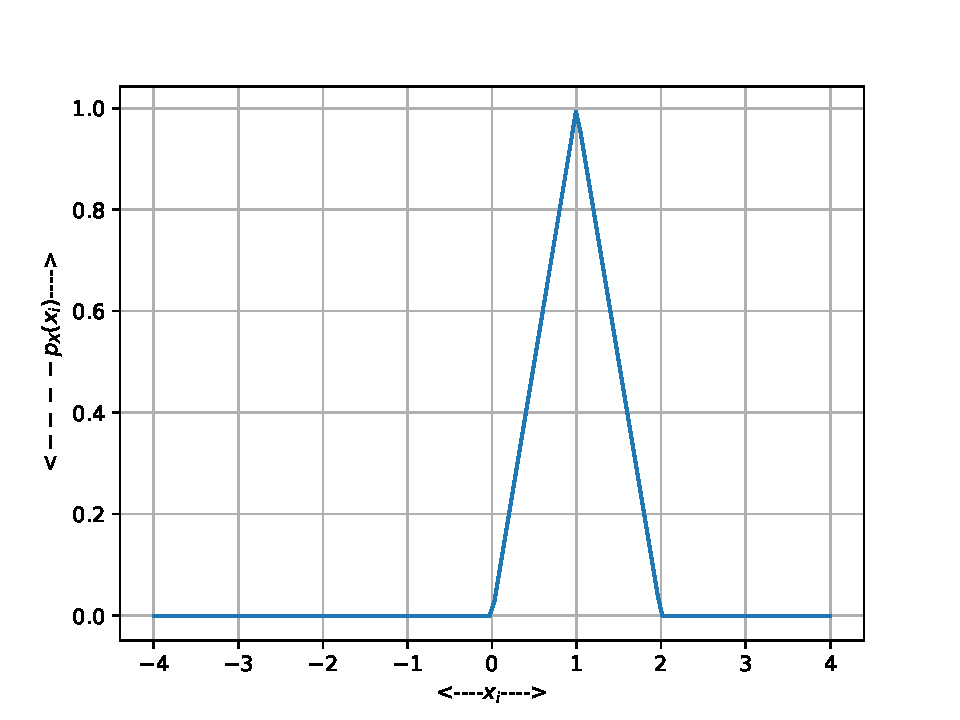
\includegraphics[width=\columnwidth]{./figs/chapter3/tri_dist_pdf.pdf}
\caption{The PDF of $T$}
\label{fig:tri_pdf}
\end{figure}

\item Verify your results through a plot. \\
\solution Verified in the above figures.
\end{enumerate}
\chapter{Maximum Likelihood Detection: BPSK}

\section{\bf{Maximum Likelihood}}
\begin{enumerate}
\item Generate equiprobable $X \in \cbrak{1,-1}$.\\
\solution \\Equiprobable of $X$ is generated using the below code  \\
\textbf{Code}
\begin{lstlisting}
from numpy import random
import matplotlib.pyplot as plt
import seaborn as sns
b=random.binomial(n=1, p=0.5, size=1000)
print(b)
sns.distplot(b, hist=False, label='binomial')
plt.show()

\end{lstlisting}
\begin{lstlisting}
codes/chapter4/eq_pb.py
\end{lstlisting}
\begin{figure}[H]
\centering
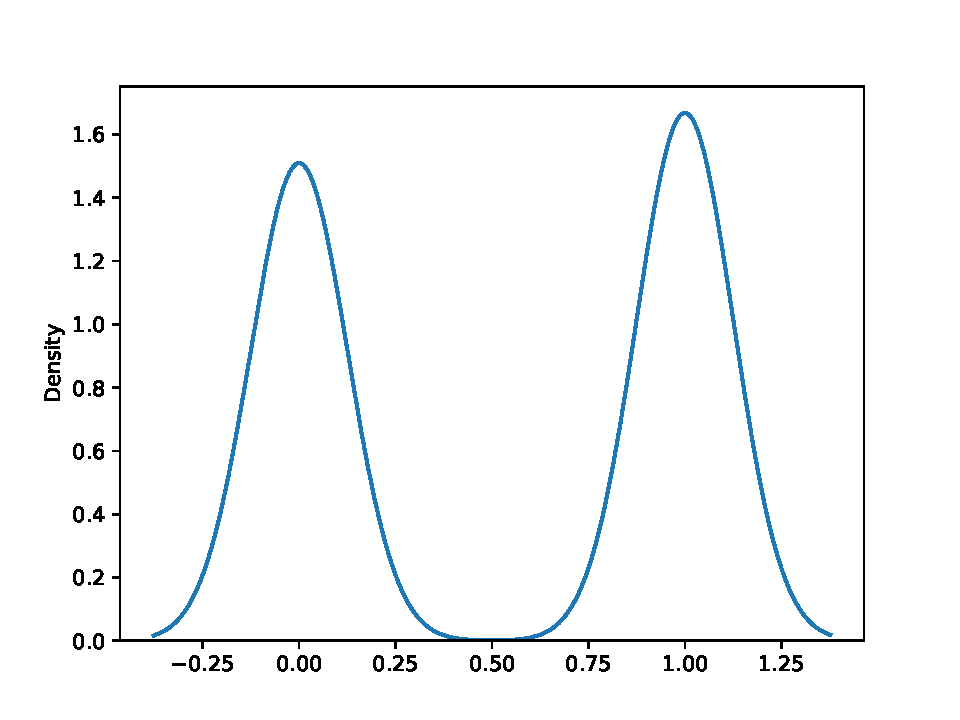
\includegraphics[width=\columnwidth]{./figs/chapter4/eq_pb.pdf}
\caption{equiprobable of  $X$}
\label{fig:eq_pb}
\end{figure}
\item Generate 
\begin{equation}
Y = AX+N,
\end{equation}
		where $A = 5$ dB,  and $N \sim \gauss{0}{1}$.\\
\solution Using the below code y can be generated.
\begin{lstlisting}[language=python]
import numpy as np
from numpy import random
import matplotlib.pyplot as plt
import seaborn as sns

n = 100
X = np.random.binomial(1, 0.5,n)*2-1
N = np.random.normal(0, 1,n)

a = 5
A = (0.1*5)**10
Y = A*X + N

sns.distplot(random.normal(loc=50, scale=5, size=1000), hist=False, label='normal')
sns.distplot(random.binomial(n=100, p=0.5, size=1000), hist=False, label='binomial')

print(Y)
plt.show()


\end{lstlisting}
Code is given below
\begin{lstlisting}
codes/chapter4/value_y.py
\end{lstlisting}
\item Plot $Y$ using a scatter plot.\\
\solution Using the below python code $Y$ can be plotted.
\begin{lstlisting}
codes/chapter4/scatter_plot_y.py
\end{lstlisting}
\begin{figure}[H]
\centering
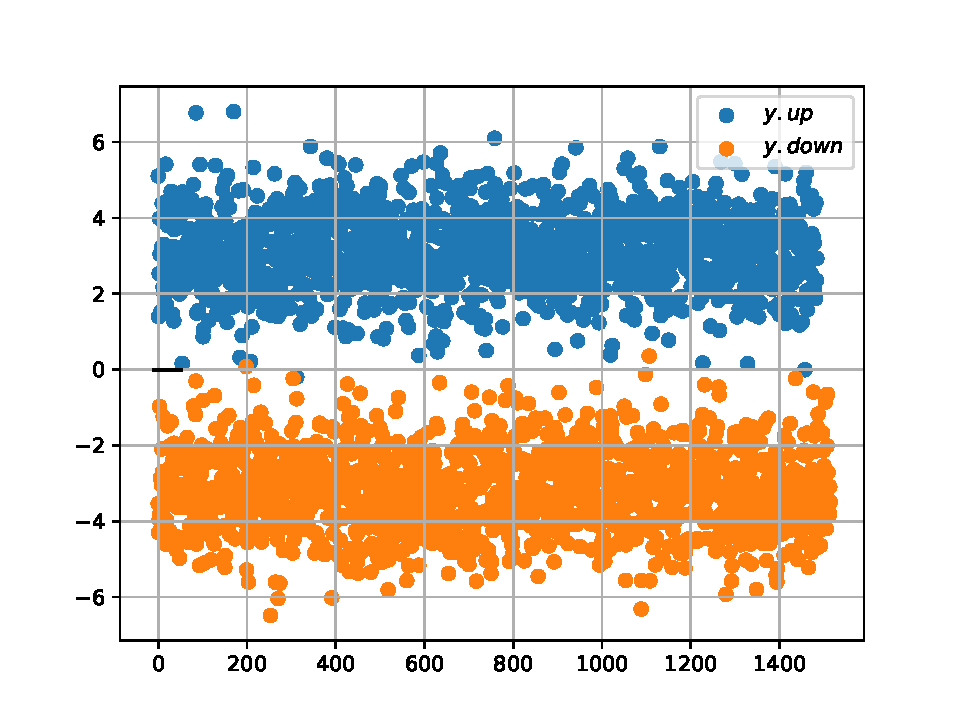
\includegraphics[width=\columnwidth]{./figs/chapter4/scatter_plot_y.pdf}
\caption{Scatter plot of $Y$}
\label{fig:bpsk_scatter}
\end{figure}
\item Guess how to estimate $X$ from $Y$.\\
\solution 
\begin{equation}
y \dec{1}{-1} 0
\end{equation}
By using the above equation we can estimate $X$ from $Y$ 
\item Find 
\begin{equation}
	P_{e|0} = \pr{\hat{X} = -1|X=1}
\end{equation}
and 
\begin{equation}
	P_{e|1} = \pr{\hat{X} = 1|X=-1}
\end{equation}\\
\solution Based on the decision rule :
\begin{equation}
y \dec{1}{-1} 0
\end{equation}
By using the above  equation\\
1. To find \begin{equation}
	P_{e|0} = \pr{\hat{X} = -1|X=1}
\end{equation}
\begin{align}
	\pr{\hat{X} = -1|X=1} 
  \end{align}
$Y < 0$ When $\hat{X} = -1$ 
 \begin{align}
        \pr{Y < 0|X=1} 
 \end{align}
         We know that $Y=AX+N$ 
\begin{align}
	 \pr{AX + N < 0|X=1}
\end{align}
  substitute $X=1$ we get
  \begin{align}
	\pr{A + N < 0}
 \end{align}
  Putting $A$ to RHS we get
  \begin{align}
	\pr{\hat{X} = -1|X=1} &= \pr{N < -A}
   \end{align} \vspace{2mm}
Similarly, \\
2. To find \begin{equation}
	P_{e|1} = \pr{\hat{X} = 1|X=-1}
\end{equation}
\begin{align}
	\pr{\hat{X} = 1|X=-1} 
  \end{align}
$Y > 0$ When $\hat{X} = 1$ 
 \begin{align}
        \pr{Y > 0|X=-1} 
 \end{align}
         We know that $Y=AX+N$ 
\begin{align}
	 \pr{AX + N > 0|X=-1}
\end{align}
  substitute $X=-1$ we get
  \begin{align}
	\pr{-A + N > 0}
 \end{align}
  Putting $A$ to RHS we get
  \begin{align}
	\pr{\hat{X} = 1|X=-1} &= \pr{N > A}
   \end{align} \vspace{2mm}
Now Since , $N \sim \gauss{0}{1}$,
\begin{align}
	 P_{e|0} = P_{e|1} &= \pr{N > A}
\end{align}
%
\item Find $P_e$ assuming that $X$ has equiprobable symbols.\\
\solution \\
By using the Q-function 
\begin{align}
	\label{eq:q_fun_ing}
	Q(x) &= \frac{1}{\sqrt{2\pi}}.\frac{1}{2} \int_x^\infty e^-u^2 \ du.
\end{align}
and Using, 
\begin{align}
	P_e = (\pr{X=1}P_{e|1}) + (\pr{X=-1}P_{e|0})
 \end{align}
	Here by question $X$ is equiprobable
    So, 
        \begin{align}
       P_r(X=\pm1) =\frac{1}{2}
        \end{align}
Substituting here,
        \begin{align}
	 P_e = \frac{1}{2} (P_{e|0} +P_{e|1})
\end{align}
Substituting it we have,
\begin{equation}
	P_e = \pr{A < N}
\end{equation}

The below equation can be written using Q-Function.
\begin{align}
    Q(A) = P_e \\
    P_e = Q(A)
\end{align} 
%
\item
Verify by plotting the theoretical $P_e$ with respect to $A$ from 0 to 10 dB.\\
\solution The theoretical $P_e$ is plotted in \figref{fig:bpsk_pe_snr}, along with numerical estimations from generated samples of $Y$. The below code is used for the plot, 
\begin{lstlisting}
codes/chapter4/theo_pe.py
\end{lstlisting}
\begin{figure}[H]
\centering
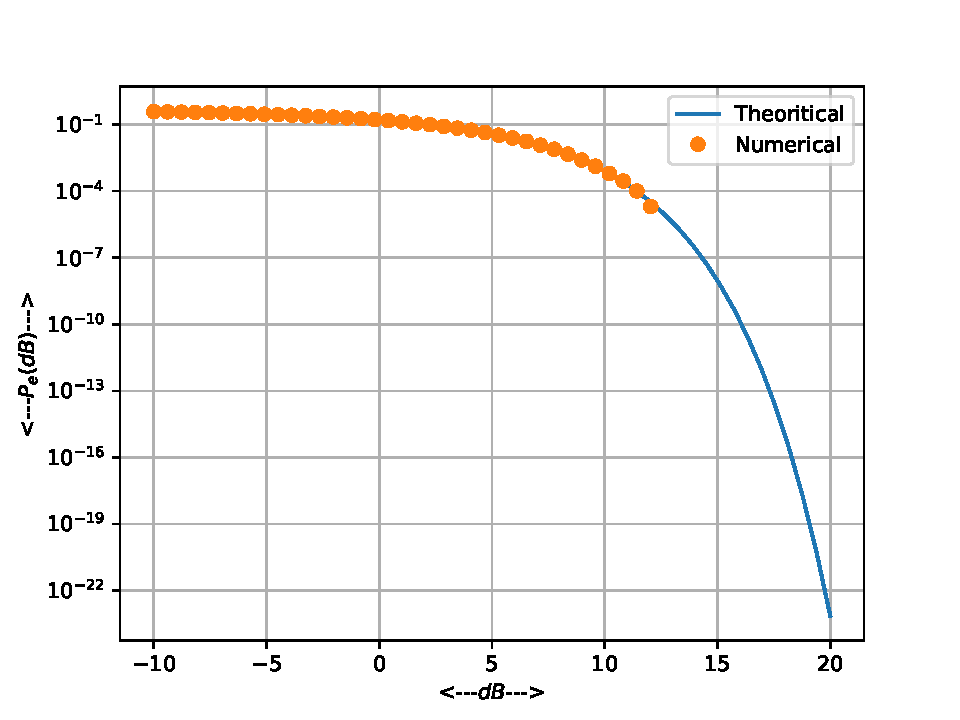
\includegraphics[width=\columnwidth]{./figs/chapter4/theo_pe.pdf}
\caption{$P_e(db)$ versus $db$ plot}
\label{fig:bpsk_pe_snr}
\end{figure}
%
\item Now, consider a threshold $\delta$  while estimating $X$ from $Y$. Find the value of $\delta$ that maximizes the theoretical $P_e$.\\
\label{prob:bpsk_delta_equi}
\solution \\
Using decision rule,
\begin{equation}
y \dec{1}{-1} \delta
\end{equation}
We have,
 \begin{equation}
	P_{e|0} = \pr{\hat{X} = -1|X=1}
\end{equation}
\begin{align}
	\pr{\hat{X} = -1|X=1} 
  \end{align}
$Y < 0$ When $\hat{X} = -1$ 
 \begin{align}
        \pr{Y < 0|X=1} 
 \end{align}
         We know that $Y=AX+N$ 
\begin{align}
	 \pr{AX + N < 0|X=1}
\end{align}
  substitute $X=1$ we get
  \begin{align}
	\pr{A + N < 0}
 \end{align}
  Putting $A$ to RHS we get
  \begin{align}
	\pr{\hat{X} = -1|X=1} &= \pr{N < -A}
   \end{align} \vspace{2mm}
   Now replacing zero as $\delta$ 
   We get,
   \begin{align}
       \pr{Y < \delta|X=1}&\\
       \pr{A + N < \delta} \\
        \pr{N < -A + \delta}&\\
         Q(A-\delta)
\end{align}
Therefore 
\begin{align}
    P_{e|1}=Q(A-\delta)
\end{align}
Similarly, 
\begin{equation}
	P_{e|1} = \pr{\hat{X} = 1|X=-1}
\end{equation}
\begin{align}
	\pr{\hat{X} = 1|X=-1} 
  \end{align}
$Y > 0$ When $\hat{X} = 1$ 
 \begin{align}
        \pr{Y > 0|X=-1} 
 \end{align}
         We know that $Y=AX+N$ 
\begin{align}
	 \pr{AX + N > 0|X=-1}
\end{align}
  substitute $X=-1$ we get
  \begin{align}
	\pr{-A + N > 0}
 \end{align}
  Putting $A$ to RHS we get
  \begin{align}
	\pr{\hat{X} = 1|X=-1} &= \pr{N > A}
   \end{align} 
   Similarly, replacing zero as $\delta$ \\
   We have,
\begin{align}
	P_{e|1} \pr{\hat{X} = 1|X=-1}\\
	\pr{Y > \delta|X=-1}\\
	\pr{N > A + \delta}\\
	Q(A+\delta)
 \end{align}
 Therefore
 \begin{align}
     P_{e|0}=Q(A+\delta)
     \end{align}
Using the below equation 
 \begin{align}
	 P_e = \frac{1}{2} (P_{e|0} +P_{e|1})
\end{align}
Using the above $P_{e|0}$ and $P_{e|1}$ values $P_e$ is written as,
\begin{flalign}
	P_e &= \frac{1}{2}Q(A+\delta) + \frac{1}{2}Q(A-\delta)
\end{flalign}
Using the integral for Q-function from \eqref{eq:q_fun_ing},
\begin{align}
	Q(x) &= \frac{1}{\sqrt{2\pi}}.\frac{1}{2} \int_x^\infty e^-u^2 \ du.
\end{align}
$P_e$ can be written as,
\begin{align}
	\label{eq:delta_eq}
	P_e &= k(\int_{A+\delta}^\infty \exp\left(-\frac{u^2}{2}\right)du  + \int_{A-\delta}^\infty \exp\left(-\frac{u^2}{2}\right) \, du)\ 
 \end{align}
where k is a constant	\\
By Differentiating the above equation \eqref{eq:delta_eq} wrt $\delta$ ,\\
we get
\begin{align}
   \frac{dP_e}{d\delta}= \exp\left(-\frac{(A+\delta)^2}{2}\right)-\exp\left(-\frac{(A-\delta)^2}{2}\right) d\delta.
\end{align}
By equating it to zero we get,
\begin{flalign*}
	\exp\left(-\frac{(A+\delta)^2}{2}\right)-\exp\left(-\frac{(A-\delta)^2}{2}\right) &= 0&\\
	-\exp\left(\frac{(A+\delta)^2-(A-\delta)^2}{2}\right) &= 1&\\
	\exp\left(-2A\delta\right) &= 1&\\
	\intertext{Therefore}\\
	\delta &= 0
\end{flalign*}
For $\delta=0$ $P_e$ is maximum. 
\item Repeat the above exercise when 
	\begin{align}
		p_{X}(0) = p
	\end{align}
\solution \\
We know that
\begin{align}
	P_e = (\pr{X=1}P_{e|1}) + (\pr{X=-1}P_{e|0})
 \end{align}
 Now $P_{e|1}$ and $P_{e|0}$ is defined as,
 \begin{align}
     P_{e|1}=Q(A+\delta) \\
      P_{e|0}=Q(A-\delta)
 \end{align}
 Since non equiprobabl $X$ is defined as
 \begin{align}
    \pr{X=1}=(1-p) \\
    \pr{X=-1}=p
 \end{align}
From the above equation and Since $X$ is not equiprobable, $P_e$ is given by,
\begin{flalign}
	P_e =& (1-p)P_{e|1} + pP_{e|0}\\
	P_e =& (1-p)Q(A+\delta) + pQ(A-\delta)
\end{flalign}
Using the integral for Q-function 
\begin{align}
	Q(x) &= \frac{1}{\sqrt{2\pi}}.\frac{1}{2} \int_x^\infty e^-u^2 \ du.
\end{align}

From \eqref{eq:delta_eq} $P_e$ can be defined as
$P_e$ can be written as, 
\begin{align}
	\label{eq:delta_eq}
	P_e &= k(\int_{A+\delta}^\infty \exp\left(-\frac{u^2}{2}\right)du  + \int_{A-\delta}^\infty \exp\left(-\frac{u^2}{2}\right) \, du)\ 
 \end{align}

 Using the above equation we can write for $p_{X}(0) = p$
\begin{multline}
	P_e = \left(k((1-p)\int_{A+\delta}^\infty \exp\left(-\frac{u^2}{2}\right) \, du \right) + \\
	\left( p\int_{A-\delta}^\infty \exp\left(-\frac{u^2}{2}\right) \, du \right)
\end{multline}
$k$ is a constant.\\
Differentiate $P_e$ wrt $\delta$ and equate to zero\\
We have 
\begin{align}
   \frac{dP_e}{d\delta}= (1-p)\exp\left(-\frac{(A+\delta)^2}{2}\right)-p\exp\left(-\frac{(A-\delta)^2}{2}\right) d\delta.
\end{align}
Following the same steps as in problem \ref{prob:bpsk_delta_equi}, $\delta$ for maximum $P_e$ evaluates to,
\begin{equation}
	\delta = \frac{1}{2A}\ln\left(\frac{1}{p}-1\right)
\end{equation}
Equating the above equation to zero
\begin{flalign*}
	(1-p)\exp\left(-\frac{(A+\delta)^2}{2}\right)-(p)\exp\left(-\frac{(A-\delta)^2}{2}\right) = 0\\
	\exp\left(-\frac{(A+\delta)^2-(A-\delta)^2}{2}\right) = \frac{p}{(1-p)} \\
	\exp\left(-2A\delta\right) = \frac{p}{(1-p)}\\
	\intertext{Therefore}\\
	\delta = \frac{1}{2A} \log \left(\frac{1}{p}-1\right)
\end{flalign*}
\end{enumerate}
%-----next chapter------%
\chapter{Transformation of Random Variables}
\section{Gaussian to Other}
\begin{enumerate}
\item
Let $X_1 \sim  \gauss{0}{1}$ and $X_2 \sim  \gauss{0}{1}$. Plot the CDF and PDF of
%
\begin{equation}
V = X_1^2 + X_2^2
\end{equation}\\
\solution \\
Below code gives CDF of V.
\begin{lstlisting}
codes/chapter5/sum_cdf
\end{lstlisting}
\begin{figure}[H]
\centering
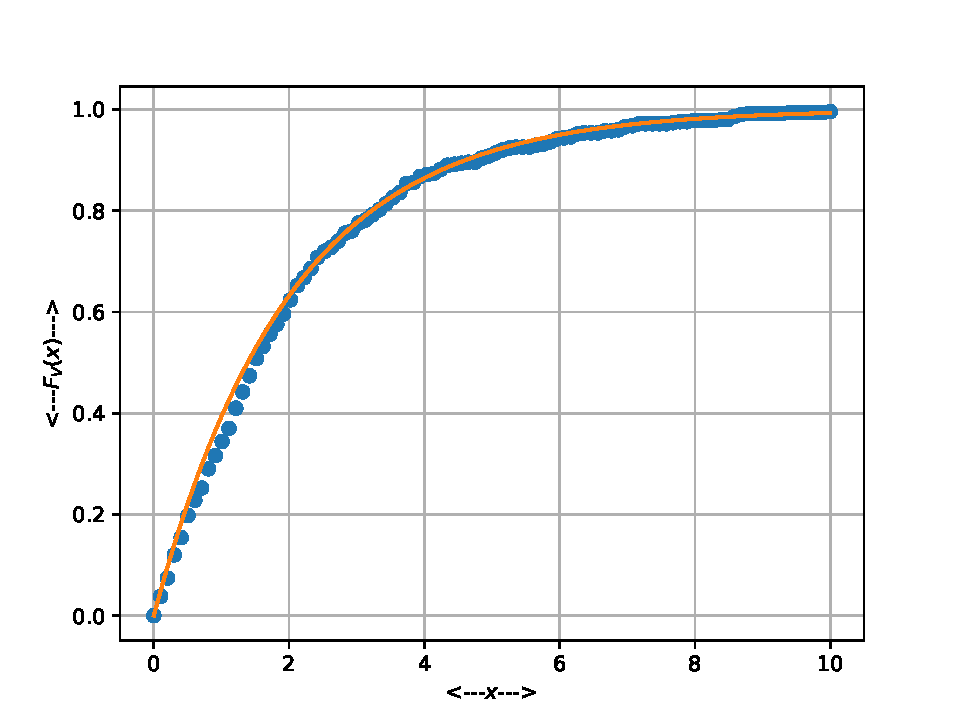
\includegraphics[width=\columnwidth]{./figs/chapter5/sum_cdf.pdf}
\caption{CDF of $V$}
\end{figure}
Below code gives PDF of V.
\begin{lstlisting}
codes/chapter5/sum_pdf
\end{lstlisting}
\begin{figure}[H]
\centering
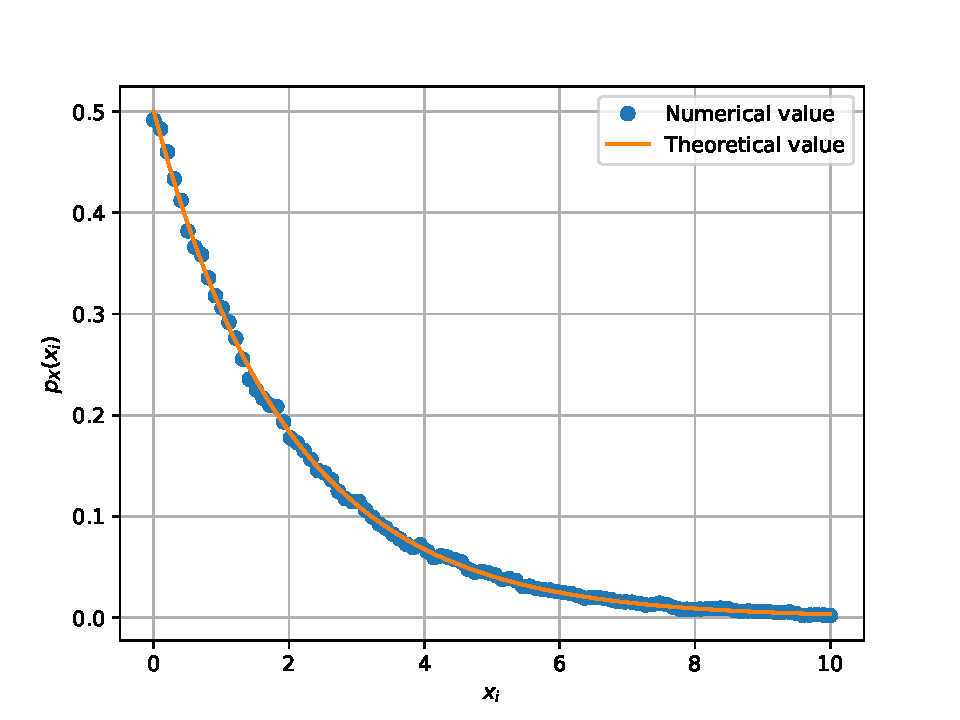
\includegraphics[width=\columnwidth]{./figs/chapter5/sum_pdf.pdf}
\caption{PDF of $V$}
\end{figure}
%
%
%
\item
If
%
\begin{equation}
F_{V}(x) = 
\begin{cases}
1 - e^{-\alpha x} & x \geq 0 \\
0 & x < 0,
\end{cases}
\end{equation}
%
find $\alpha$.\\
\solution \\
Below code gives CDF of V with different alfa values.
\begin{lstlisting}
codes/chapter5/value_alfa.py
\end{lstlisting}
\begin{figure}[H]
\centering
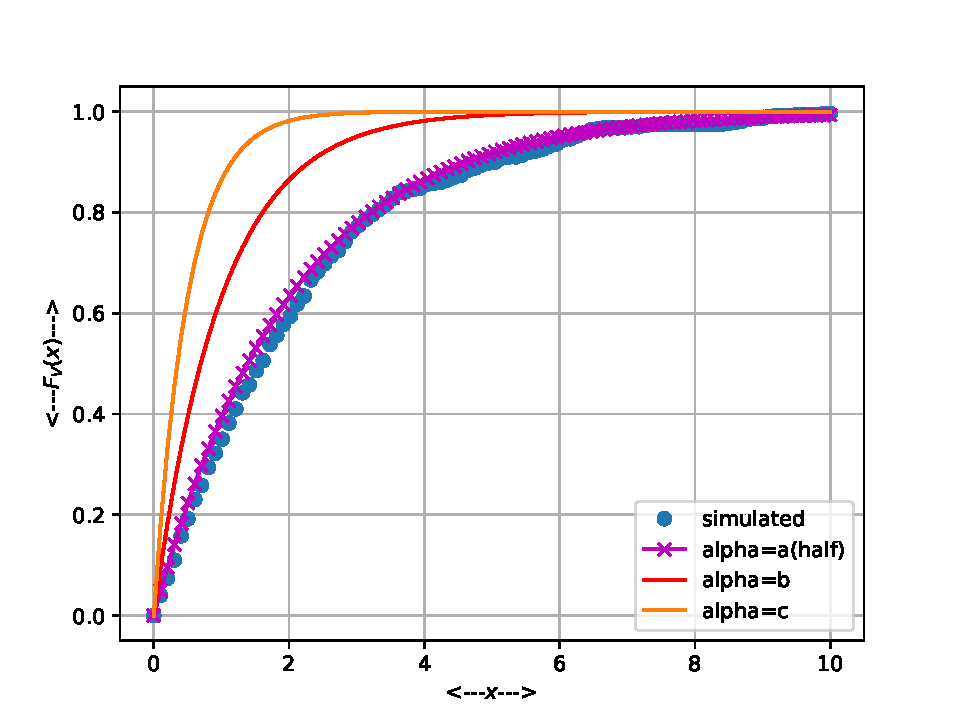
\includegraphics[width=\columnwidth]{./figs/chapter5/value_alfa.pdf}
\caption{PDF of $V$}
\end{figure}
From the above figure $\alpha = 0.5$.
%
\item
\label{ch3_raleigh_sim}
Plot the CDF and PDF of
%
\begin{equation}
A = \sqrt{V}
\end{equation}\\
\solution \\
Below code gives you CDF of A.
\begin{lstlisting}
codes/chapter5/sq_root_cdf.py
\end{lstlisting}

\begin{figure}[H]
\centering
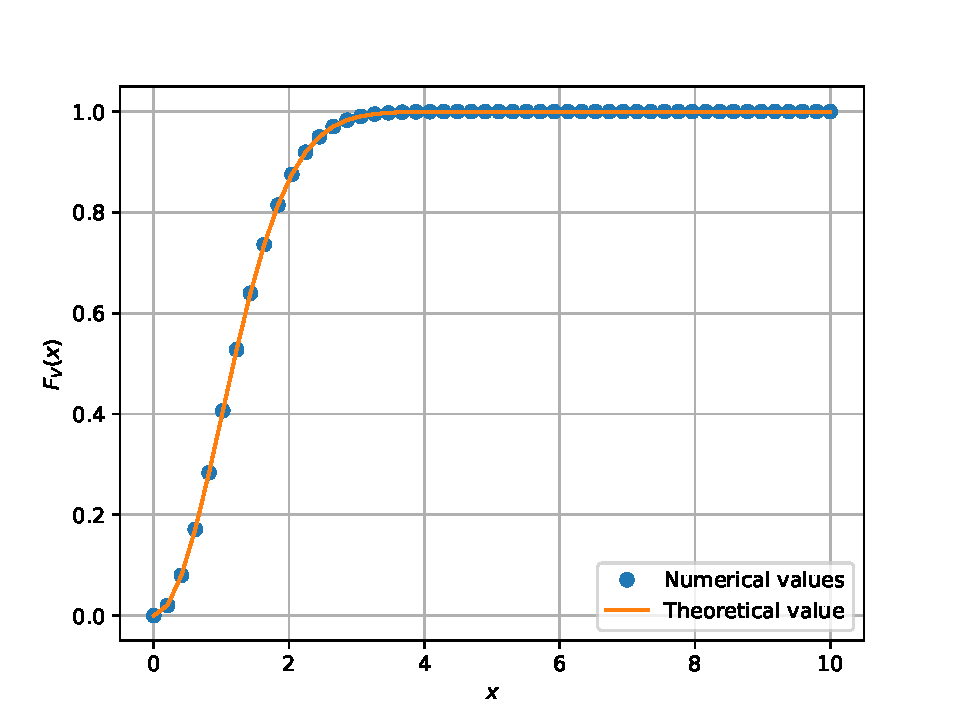
\includegraphics[width=\columnwidth]{./figs/chapter5/sqroot_cdf.pdf}
\caption{CDF of $A$}
\label{fig:rayleigh_cdf}
\end{figure}
Below code gives you CDF of A.
\begin{lstlisting}
codes/chapter5/sq_root_cdf.py
\end{lstlisting}
\begin{figure}[H]
\centering
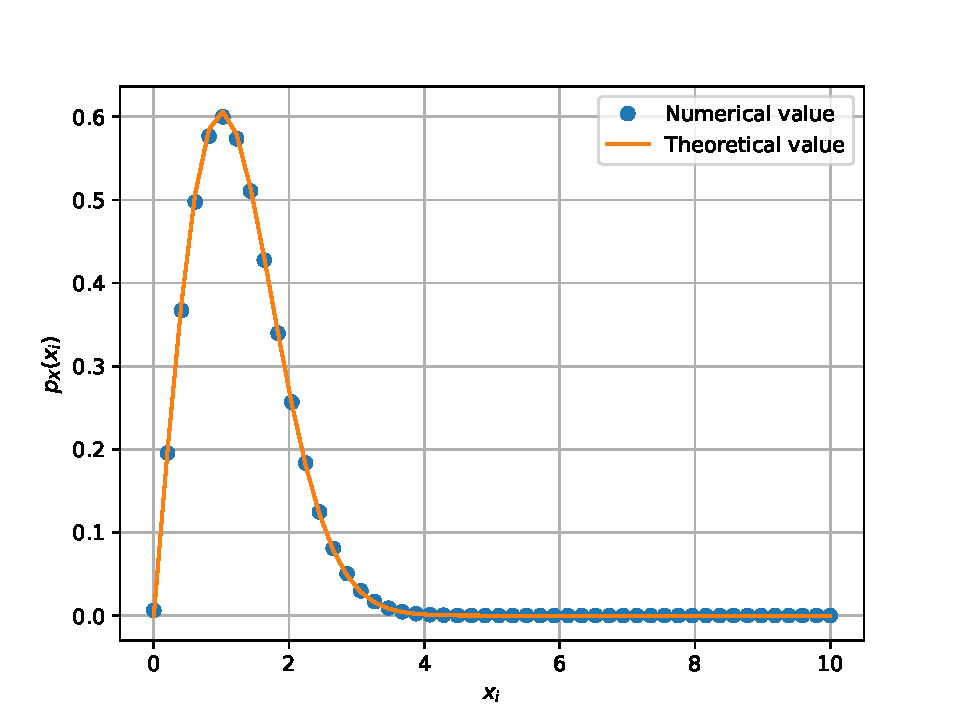
\includegraphics[width=\columnwidth]{./figs/chapter5/sqroot_pdf.pdf}
\caption{PDF of $A$}
\end{figure}
%
\end{enumerate}
%
\section{Conditional Probability}
\begin{enumerate}
\item
\label{ch4_sim}
Plot 
\begin{equation}
P_e = \pr{\hat{X} = -1|X=1}
\end{equation}
%
for 
\begin{equation}
Y = AX+N,
\end{equation}
where $A$ is Raleigh with $E\sbrak{A^2} = \gamma, N \sim \gauss{0}{1}, X \in \brak{-1,1}$ for $0 \le \gamma \le 10$ dB.\\ 
\solution In below figure the dots are required values \\
Below code gives the plot of $P_e$
\begin{lstlisting}
codes/chapter5/value_pe.py
\end{lstlisting}
\begin{figure}[H]
\centering
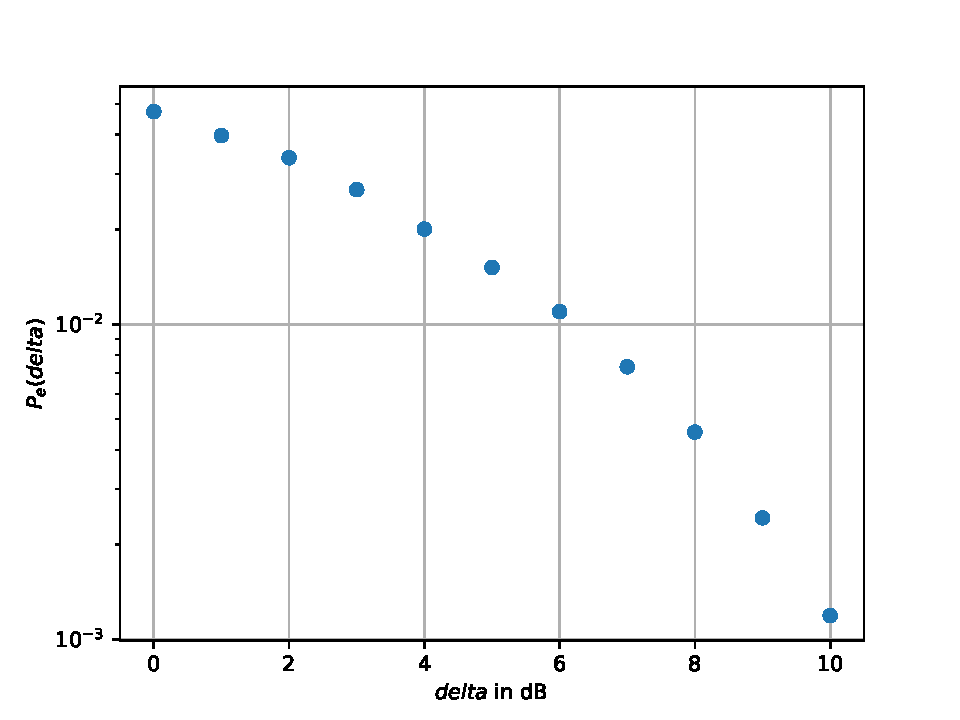
\includegraphics[width=\columnwidth]{./figs/chapter5/value_pe.pdf}
\caption{Value Of $P_e$ }
\end{figure}
%
\item
Assuming that $N$ is a constant, find an expression for $P_e$.  Call this $P_e(N)$\\
\solution\\
The value of $P_e$ is given by,
\begin{align}
    P_e &= \pr{\hat{X} = -1|X=1}&\\ \nonumber
\end{align}

\begin{equation}
	 \hat X=
	\begin{cases} 
	-1 & N < -A\\
	1 & N > A
	\end{cases}
\end{equation}
For $\hat X=-1$ $Y<0$ always and $Y=AX+N$ 
\begin{align}
     P_e &=\pr{AX+N<0|X=1}\\
     P_e &=\pr{A+N<0}&\text{for X=1}\\ \nonumber 
     P_e &= \pr{A<-N}\\
\end{align}
The $P_e$ is defind wrt constant $N$ 

\begin{equation}
\label{eq:Pe_value}
P_e(N)=\begin{cases}
	F_X(N) & N \ge 0\\
	0 & N < 0
	\end{cases}
\end{equation}

For random variable $X$ with $E\sbrak{X^2} = \gamma$, CDF is given by
\begin{align}
	\label{eq:x_cdf}
	F_X(x) &= 1-\exp\left(-\frac{X^2}{\gamma}\right) \text{ for } x \ge 0
\end{align}
Substituting \eqref{eq:x_cdf} in \eqref{eq:Pe_value},
\begin{equation}
	P_e(N) =
	\begin{cases} 
	1-\exp\left(-\frac{N^2}{\gamma}\right) & N \ge 0\\
	0 & N < 0
	\end{cases}
\end{equation}
%or 
\begin{center}
    or
\end{center}
When $N < 0$

\begin{equation}
 P_e(N) = \int_{-\infty}^{N}F_X(x)\, dx \int_{-\infty}^{0}\, dx + \int_{0}^{N}F_X(x)\, dx\\
\end{equation}
\begin{equation}
 P_e(N) = \int_{0}^{N}\frac{x}{\sigma^2} \exp \left(\frac{-x^2}{2\sigma^2}\right)\, dx \\
\end{equation}
Now $P_e$(N) is defined as,
\begin{equation}
    P_e(N) =
	\begin{cases} 
	1-\exp\left(-\frac{N^2}{2\sigma^2}\right) & N \ge 0\\
	0 & N < 0
	\end{cases}
\end{equation}
\item
%
\label{ch4_anal}
For a function $g$,
\begin{equation}
E\sbrak{g(X)} = \int_{-\infty}^{\infty}g(x)p_{X}(x)\, dx
\end{equation}
%
Find $P_e = E\sbrak{P_e(N)}$.\\
\solution\\
Using $P_e(N)$ from \eqref{eq:Pe_value} 
\begin{equation}
	P_e(N) =
	\begin{cases} 
	1-\exp\left(-\frac{N^2}{\gamma}\right) & N \ge 0\\
	0 & N < 0
	\end{cases}
\end{equation}
and We know that, 
\begin{align}
    P_N(x)=\frac{1}{\sqrt{2}\pi}\exp\left(\frac{-x^2}{2}\right)
\end{align}
\begin{flalign*}
	P_e =E\sbrak{P_e(N)}&= \int_{-\infty}^{\infty} P_e(x)p_N(x) \,dx&\\
	&= \int_{0}^{\infty} \left(1-e^{-\frac{x^2}{\gamma}}\right)\frac{1}{\sqrt{2\pi}}e^{-\frac{x^2}{2}} \,dx
\end{flalign*}
	
\begin{equation}
	P_e =  \frac{1}{\sqrt{2\pi}}\int_{0}^{\infty} e^{-\frac{x^2}{2}}  \,dx
\end{equation}
By integrating the above equation.\\
We get
\begin{flalign*}
	P_e &= \frac{1}{2} - \frac{1}{2}\sqrt{\frac{\gamma}{2+\gamma}}
\end{flalign*} 
%
\item
Plot $P_e$ in problems \ref{ch4_sim} and \ref{ch4_anal} on the same graph w.r.t $\gamma$.  Comment.\\
\solution\\
Below code gives you CDF of A.
\begin{lstlisting}
codes/chapter5/value_pe_del.py
\end{lstlisting}
\begin{figure}[H]
\centering
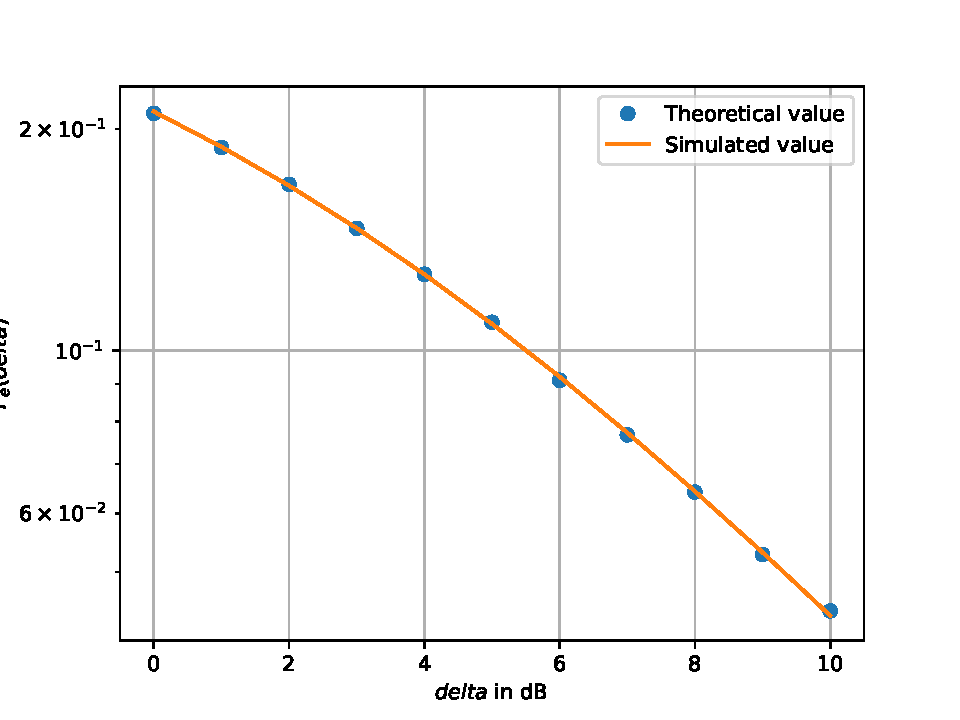
\includegraphics[width=\columnwidth]{./figs/chapter5/value_pe_del.pdf}
\caption{$P_e$ versus $\gamma$}
\label{fig:bpsk_pe_snr_rayleigh}
\end{figure}
\end{enumerate}
%
\end{document}